\section{Results}

We represent each \Cyclus result as a solid line, and the benchmark solution
as a dotted line for visualization. The results are
simply a reproduction of the plots displayed in the benchmark. 
We obtained the benchmark solutions through personal contact with
benchmark author Bo Feng at Argonne National Laboratory.



Figure \ref{fig:pow_plot} shows the deployed reactor capacity, and
figure \ref{fig:dep} shows the \gls{LWR} retirement and \gls{SFR}
deployment. The two plots show exact agreement with the
benchmark solutions.

\begin{figure}[htbp!]
    \begin{center}
        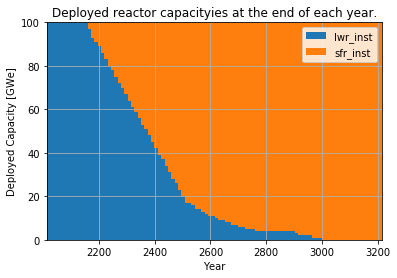
\includegraphics[scale=0.5]{./images/results_18/power_plot.png}
    \end{center}
        \caption{Deployed reactor capacities at the end of each year.}
    \label{fig:pow_plot}
\end{figure}


\begin{figure}[htbp!]
	\begin{center}
		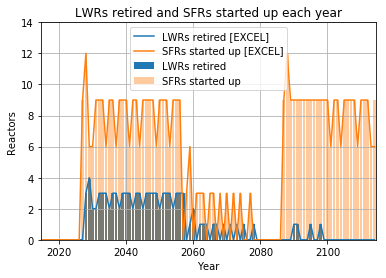
\includegraphics[scale=0.5]{./images/results_18/dep.png}
	\end{center}
        \caption{\glspl{LWR} retired and \glspl{SFR} started up each year.}
	\label{fig:dep}
\end{figure}

Figure \ref{fig:fuel_load} shows the annual fuel loading rate.
The initial fuel loading for 100 \gls{LWR} reactors was edited to match
the plot in the verification
study results. The oscillations caused by the 18 month refueling period
were aggregated into 12 month groups. As a result the total fuel loaded
are equal for both plots.

Although indistinguishable in figure \ref{fig:fuel_load},
there is a small difference between \gls{SFR} fuel loading proportional
to the core mass difference, as mentioned in the previous section.
Figure \ref{fig:fuel_load_diff_norm} shows the
differences normalized by the core mass differences, overlapped with the
\gls{SFR} deployment. This shows that the differences only occur during
deployment due to the difference in core mass.


\begin{figure}[htbp!]
    \begin{center}
        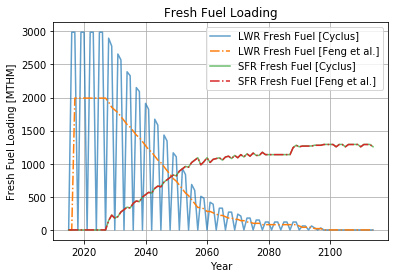
\includegraphics[scale=0.5]{./images/results_18/fuel_load.png}
    \end{center}
        \caption{Annual fresh fuel loading rates (first cores and reload fuel).}
    \label{fig:fuel_load}
\end{figure}

Figure \ref{fig:fuel_discharge_monthly} shows the inventory of discharged
\gls{UNF} in the mandatory cooling stage (four years for \gls{LWR}, one year for \gls{SFR}).
It also oscillates between the benchmark's
solution and converges, caused by the influx and the outflux of \gls{UNF}
into and out of the storage facility.
The \gls{SFR} inventory and fuel loading
solutions exactly matches the benchmark solutions, minus the small ($1.07\%$) difference due to core
size.

\begin{figure}[htbp!]
    \begin{center}
        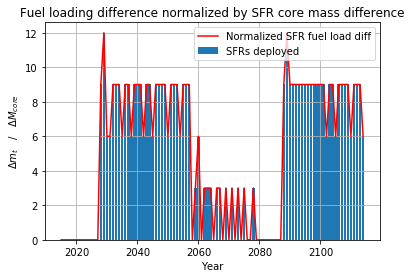
\includegraphics[scale=0.5]{./images/results_18/fuel_load_diff_norm.png}
    \end{center}
        \caption{Difference between annual fresh \gls{SFR} fuel loading rates (Cyclus - Benchmark) normalized by the core mass difference of an \gls{SFR} due to fractional batch size.}
    \label{fig:fuel_load_diff_norm}
\end{figure}


Figure \ref{fig:waiting_monthly} shows the amount of cooled \gls{UNF} waiting for
reprocessing. The value is calculated by subtracting the cumulative difference between
the cooled inventory and the \gls{UNF} reprocessing throughput.
The oscillation is between the cooled inventory in the storage facility before (high)
and after (low) it sends its inventory for reprocessing.

\begin{figure}[htbp!]
    \begin{center}
        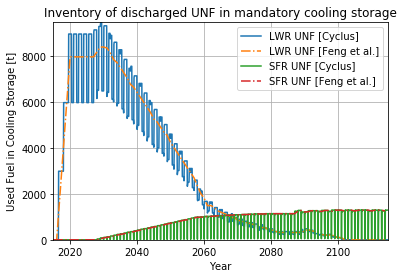
\includegraphics[scale=0.5]{./images/results_18/fuel_discharge_monthly.png}
    \end{center}
        \caption{Inventory of discharged \gls{UNF} in mandatory cooling storage.}
    \label{fig:fuel_discharge_monthly}
\end{figure}


\begin{figure}[htbp!]
    \begin{center}
        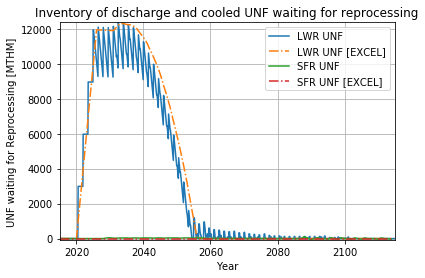
\includegraphics[scale=0.5]{./images/results_18/waiting_monthly.png}
    \end{center}
        \caption{Inventory of discharged and cooled \gls{UNF} waiting for reprocessing.}
    \label{fig:waiting_monthly}
\end{figure}


Figure \ref{fig:rep} shows the reprocessing throughput, which oscillates around
the benchmark solution. No oscillation exists in the beginning because the
\gls{LWR} \gls{UNF} reprocessing plant throughput peaks at 2,000 tons per year.

\begin{figure}[htbp!]
    \begin{center}
        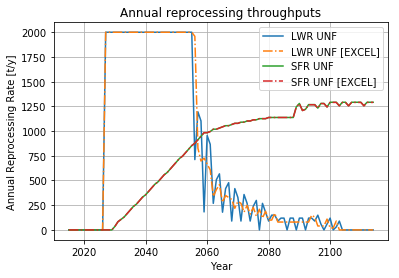
\includegraphics[scale=0.5]{./images/results_18/rep.png}
    \end{center}
        \caption{Annual reprocessing throughputs.}
    \label{fig:rep}
\end{figure}


Figure \ref{fig:tru} shows the inventory of unused \gls{TRU} recovered from \gls{UNF}.
The \Cyclus results follow the benchmark solutions closely. However,
the larger \gls{SFR} core size causes \Cyclus results to be smaller than the benchmark results,
since more \gls{TRU} is used to
start up the newly deployed \glspl{SFR}. The difference decreases as the
\glspl{SFR} decommission, discharging more \gls{UNF} (and hence \gls{TRU}) than
the benchmark.

\begin{figure}[htbp!]
	\begin{center}
		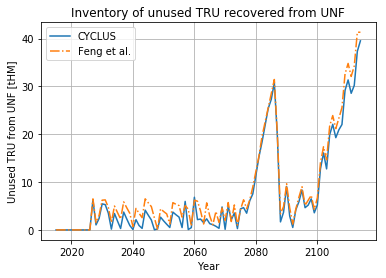
\includegraphics[scale=0.5]{./images/results_18/tru.png}
	\end{center}
        \caption{Inventory of unused \gls{TRU} recovered from \gls{UNF}.}
	\label{fig:tru}
\end{figure}

